\chapter{电路图设计}
本章节将给出NORM指令的几个主要子模块的电路图设计,包括基本的与门、或门、反向器、多位选择器、LZC模块等。

图\ref{fig2.1}所示为主要单元的电路图设计。
\begin{figure}[!hbtp]
\centering
\subfigure[基本单元或非门]{
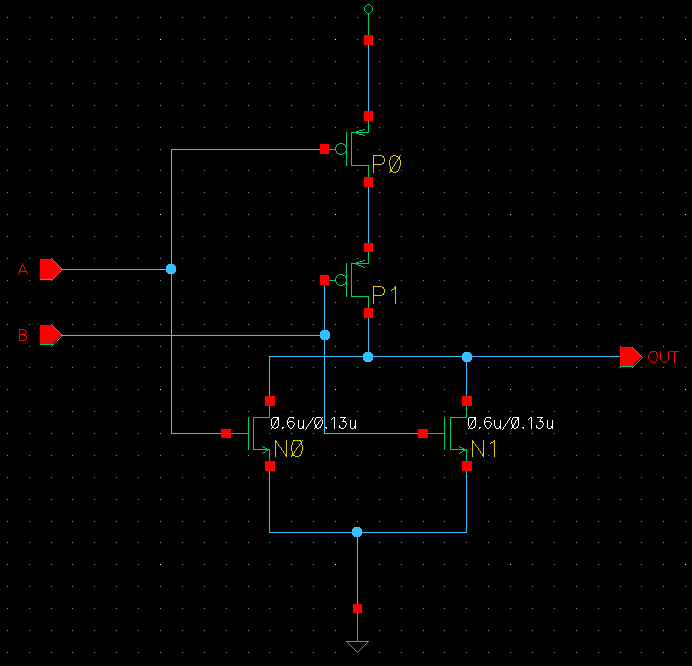
\includegraphics[width=0.4\textwidth]{chapter2/NOR}
\label{fig2.1a}
}

\subfigure[31位反向器]{
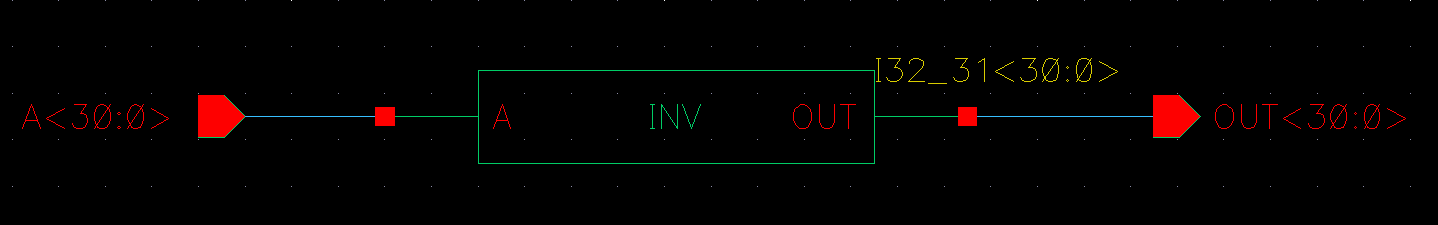
\includegraphics[width=0.4\textwidth]{chapter2/INV31}
\label{fig2.1b}
}

\subfigure[与或模块]{
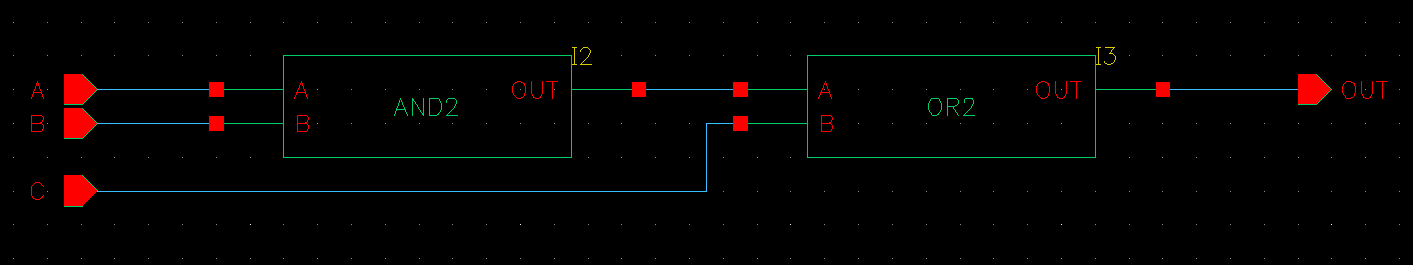
\includegraphics[width=0.4\textwidth]{chapter2/IAO}
\label{fig2.1c}
}

\subfigure[两路选择器]{
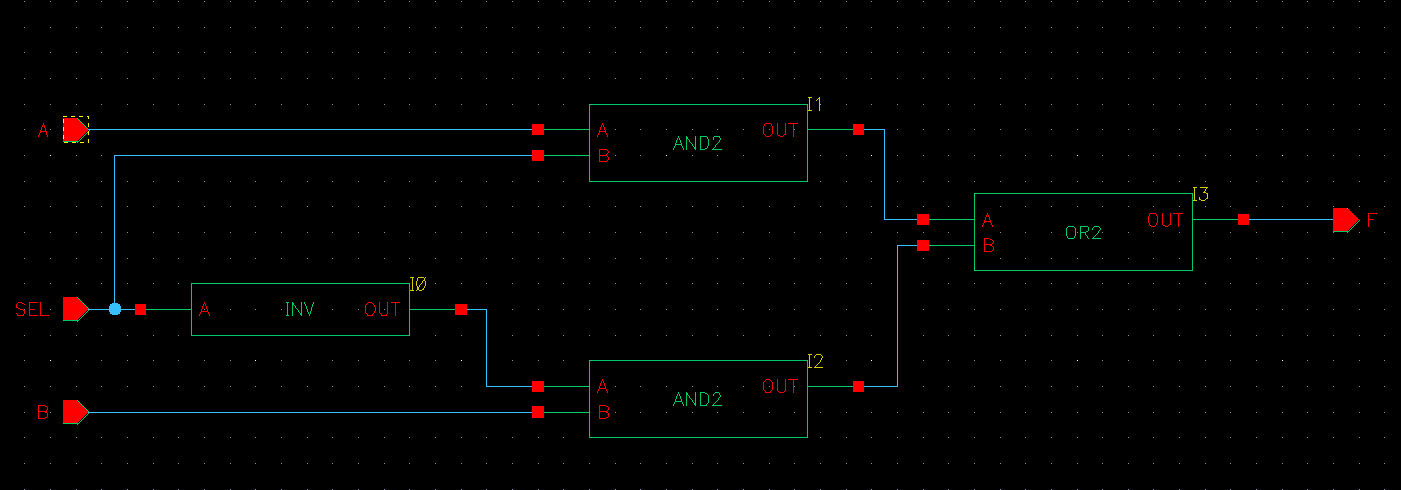
\includegraphics[width=0.4\textwidth]{chapter2/MUX2_1}
\label{fig2.1d}
}
\caption{主要基本单元的电路图设计}
\label{fig2.1}
\end{figure}\\
图\ref{fig2.2}为LZC模块的电路图设计,包括4-bit、16-bit、32-bit等不同层次。
\begin{figure}[!hbtp]
\centering
\subfigure[4-bit LZC模块]{
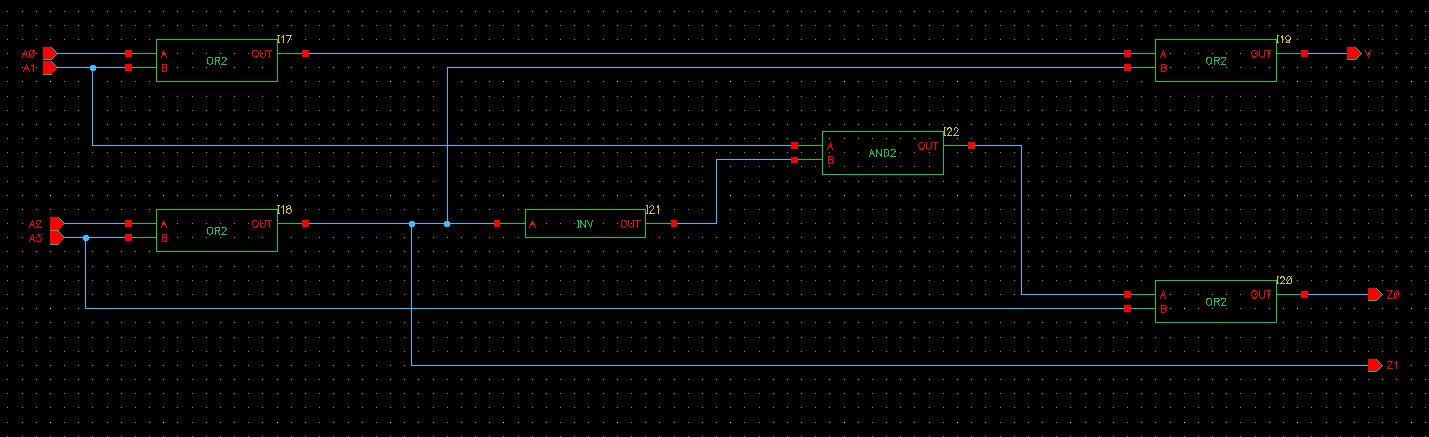
\includegraphics[width=0.6\textwidth]{chapter2/LZD4}
\label{fig2.2a}
}

\subfigure[16-bit LZC模块]{
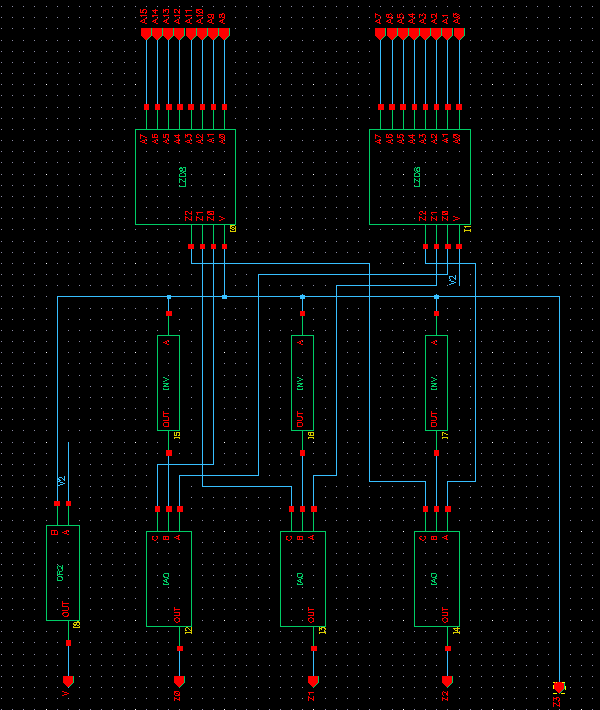
\includegraphics[width=0.5\textwidth]{chapter2/LZD16}
\label{fig2.2b}
}

\subfigure[32-bit LZC模块]{
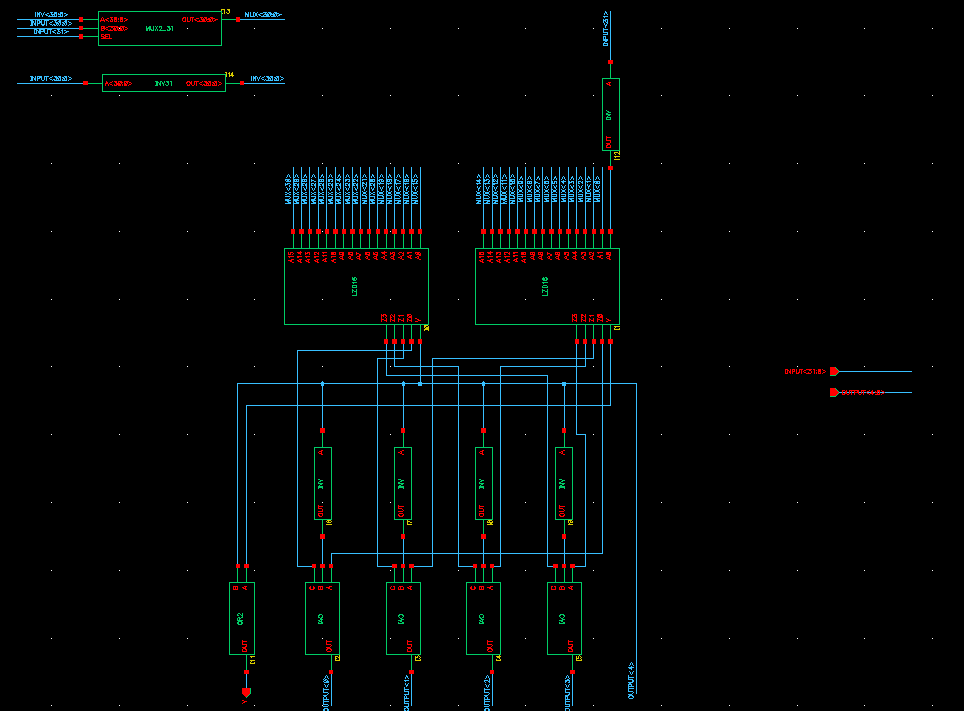
\includegraphics[width=0.65\textwidth]{chapter2/LZDF}
\label{fig2.2c}
}
\caption{主要基本单元的电路图设计}
\label{fig2.2}
\end{figure}\\
从图\ref{fig2.2}可以看出,32位LZC模块可由两个16-bit LZC子模块构成,此外还包括一个两路31位选择器,选择信号为输入操作数的符号位。需要注意的是,图\ref{fig2.2c}所示的模块的输出为6为,其中包括5位的LZC计算结果,还有1位信号$V$用于支持更宽的操作数。图\ref{fig2.3}为基于32位LZC模块以及NORM指令的功能要求实现的最终的电路图。此时,输出信号$V$被接地,且LZC计算结果被扩展为32位,高位($Lzc<31:5>$)通过27个反向器置零。
\begin{figure}[!hbtp]
\centering
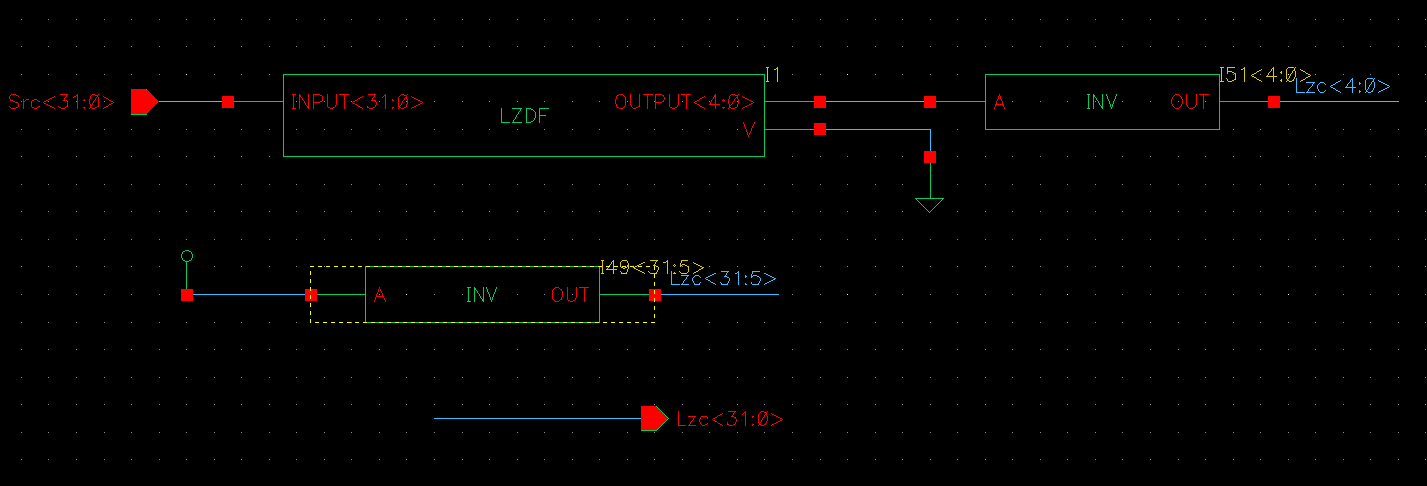
\includegraphics[width=0.9\textwidth]{chapter2/NORM}
\caption{NORM指令的实现电路}
\label{fig2.3}
\end{figure}

电路图中所有单元用到的NMOS、MPOS器件的长度均设为0.13um,NMOS的宽度设为0.6um,PMOS的宽度设为0.8um。

